% Created 2014-12-17 Wed 16:24
\documentclass[11pt]{template/openetcs_report}
\usepackage{fixltx2e}
\usepackage{graphicx}
\usepackage{longtable}
\usepackage{float}
\usepackage{wrapfig}
\usepackage{rotating}
\usepackage[normalem]{ulem}
\usepackage{amsmath}
\usepackage{textcomp}
\usepackage{marvosym}
\usepackage{wasysym}
\usepackage{amssymb}
\usepackage{hyperref}
\tolerance=1000
\usepackage{todonotes}
\usepackage{pdfpages}
\hypersetup{
  pdfkeywords={},
  pdfsubject={},
  linkbordercolor 	= {1 1 1},
  pdfcreator={Emacs 24.3.1 (Org mode 8.2.4)}}
%===========================
% Graphicpath
%===========================
\graphicspath{{./template/}{.}{./images/}}
%===========================
% Todo note margin
%===========================
\setlength{\marginparwidth}{7em}
%\let\oldmarginpar\marginpar
%\renewcommand\marginpar[1]{\-\oldmarginpar[\raggedleft\footnotesize #1]%
%{\raggedright\footnotesize #1}}
%===========================


\begin{document}
\frontmatter
\project{openETCS}


%assign a report number here
\reportnum{OETCS/WP7/07.3.5}

%define your workpackage here
\wp{Work-Package 7: ``Toolchain''}

%set a title here
\title{OpenETCS Roadmap}

%set a subtitle here
%\subtitle{}

%set the date of the report here


\date{\today}
\title{Traceability Architecture in OpenETCS}
\subtitle{WP7 Proposition}
%define a list of authors and their affiliation here

\creatorname{Cécile Braunstein}
\creatoraffil{University Bremen}
\techassessorname{}
\techassessoraffil{}

\qualityassessorname{}
\qualityassessoraffil{}

\approvalname{}
\approvalaffil{}
\author{Cecile Braunstein}
\affiliation{University Bremen}

\author{Moritz Dorka}
\affiliation{DB}

\author{David Mentré}
\affiliation{Mitsubishi Electric R\&D Centre Europe}

\author{Raphaël Faudou}
\affiliation{Samares Engineering on behalf of ENSEEIHT}


% define the coverart
\coverart[width=350pt]{openETCS_EUPL}

%define the type of report
\reporttype{OpenETCS : Position Paper on traceability}


\begin{abstract}
%define an abstract here
This document presents a proposition to the tool chain traceability
architecture.
\end{abstract}


\maketitle
\tableofcontents

\newpage
%=============================

% The actual document starts below this line
%=============================
%Start here
%=============================
% Document Managment
%=============================
\chapter{Document Information}

\begin{tabular}{|p{4.4cm}|p{8.7cm}|}

\hline
\multicolumn{2}{|c|}{Document information} \\
\hline
Work Package &  WP7  \\
Deliverable ID or doc. ref. & O7.3.5\\
\hline
Document title &Traceability Architecture in OpenETCS \\
Document version & 00.02 \\
Document authors (org.)  & Cécile Braunstein (Uni.Bremen) \\
\hline
\end{tabular}

\begin{tabular}{|p{4.4cm}|p{8.7cm}|}
\hline
\multicolumn{2}{|c|}{Review information} \\
\hline
Last version reviewed &  \\
\hline
Main reviewers &  \\
\hline
\end{tabular}

\begin{tabular}{|p{2.2cm}|p{4cm}|p{4cm}|p{2cm}|}
\hline
\multicolumn{4}{|c|}{Approbation} \\
\hline
  &  Name & Role & Date   \\
\hline  
Written by    &  Cécile Braunstein & WP7-T7.3 Sub-Task  & 06.02.2014 \\
&  & Leader&\\
\hline
Approved by &  &   &  \\
\hline
\end{tabular}

\begin{tabular}{|p{2.2cm}|p{2cm}|p{3cm}|p{5cm}|}
\hline
\multicolumn{4}{|c|}{Document evolution} \\
\hline
Version &  Date & Author(s) & Justification  \\
\hline  
00.00 & 17.12.2014 & C. Braunstein  &  Document creation  \\
\hline  
00.00 & 23.10.2015 & R. Faudou  &  Precisions concerning OpenETCS requirements and models and update of tool chain traceability requirements  \\


\hline  
\end{tabular}
\newpage
%==========================================
\mainmatter
%----------------------
\chapter{Introduction}
\section{Document purpose}
This document presents a proposition concerning support of openETCS project traceability activity by openETCS tool chain. This proposition is a consensus between traceability needs, project policy (open source solutions), time and efforts (focus on existing tools and features) and risks about tool maturity.

\section{Document scope}
This proposition is based on the needs and priorities about traceability, captured from different work packages (mainly WP3 and WP4) during October 2015, either from interviews or from reading of available project documents, especially:
\begin{itemize} 
\item Project Quality Assurance Plan - D1.3 - \cite{qa-plan}.
\item Definition of OpenETCS Development Process - D2.3a v02 - \cite{D2.3a}
\item OpenETCS Architecture and Design Specification - D3.5.0 - \cite{D3.5.0}  and D3.5.1 - \cite{D3.5.3}
\item Safety plan - D4.2.3 - \cite{D4.2.3}
\end{itemize}

The proposition done in this document is based on existing tools and existing tool capabilities with verified maturity. Document will explain limits of current proposition and will suggest axes to investigate in the future of project (roadmap).
But detailed evaluations of tools and features based on those investigations is not part of this document.

\section{Document organization}
Chapter 2 recalls openETCS project scope, development process, different needs and requirements to address, architecture and design specification.

Chapter 3 highlights main priorities concerning traceability and detailed expectations about traceability activities to support (including design, code, verification and validation).

Chapter 4 defines tool chain requirements concerning traceability.

Chapter 5 presents current traceability architecture defined to support tool chain requirements identified in chapter 4. This architecture is based on use of existing mature tools.

Chapter 6 summarizes limits of the current traceability architecture and suggests axes to investigate in order to improve traceability support by the OpenETCS tool chain.

\chapter{OpenETCS traceability scope}

Requirement traceability concerns relations between requirements existing at different engineering levels and relations between requirements and other engineering artifacts (models, documents, test cases, code...). All those requirement traceability links can have different semantics including derivation, refinement, satisfaction, implementation and verification. 

Before defining traceability process and the different link types, it is important to clearly define the scope of openETCS activity and the requirements that we want to trace. Next paragraphs recall OpenETCS vision, design process and VV process.

\section{Recall of OpenETCS target vision and development process}
\label{OpenETCS scope}
\cite{D2.3a} mentions that openETCS activity pursues the vision of a full CENELEC compliant development of open-source software for the \emph{European Vital   Computer} (EVC). It is intended to produce a software kernel which can be used in commercial EVCs.

CENELEC 50128:2011 is the relevant engineering standard for software development of safety-critical rail systems. It is completed with CENELEC 50126-1:1999 to address system and subsystem engineering activities required to prepare software development with system requirements. 


\cite{D4.2.3} recalls that \textit{the main products of the openETCS project will be the openETCS specification model used to generate the openETCS on-board software and the openETCS tool chain development, which is used to formalize the ERA Specifications for ETCS, generate the Software Code and perform verification and validation activities} 

OpenETCS software development process reflects this model-based approach while remaining compliant with CENELEC engineering standards. 

\begin{figure} [htbp]
\centering
\includegraphics[width=.9\linewidth]
{./images/OpenETCSDevelopmentProcess.png}
\caption{\label{fig:OpenETCSDevelopmentProcess}OpenETCS software development process}
\end{figure} 

\section{OpenETCS project context-of-interest}
\label{OpenETCS_ITEAProjectScope}
\cite{D3.5.3} recalls last refinement of project scope concerning functional coverage: "OpenETCS project has decided not to consider all ETCS subsystems and to tailor scope to cover the functionality required for the openETCS demonstration as an objective of the ITEA2 project. The goal is to develop a formal model and to demonstrate the functionality during a proof of concept on the ETCS Level 2 Utrecht Amsterdam track with real scenarios".

Figure \ref{fig:openETCSSystemOfInterest} details ETCS system scope to consider in order to cover expected demonstration of EVC software for ITEA project. Scope is highlighted in ERA TSI chapter 2 and provides basis for System detailed analysis and functional breakdown.

\begin{figure}[htbp]
\centering
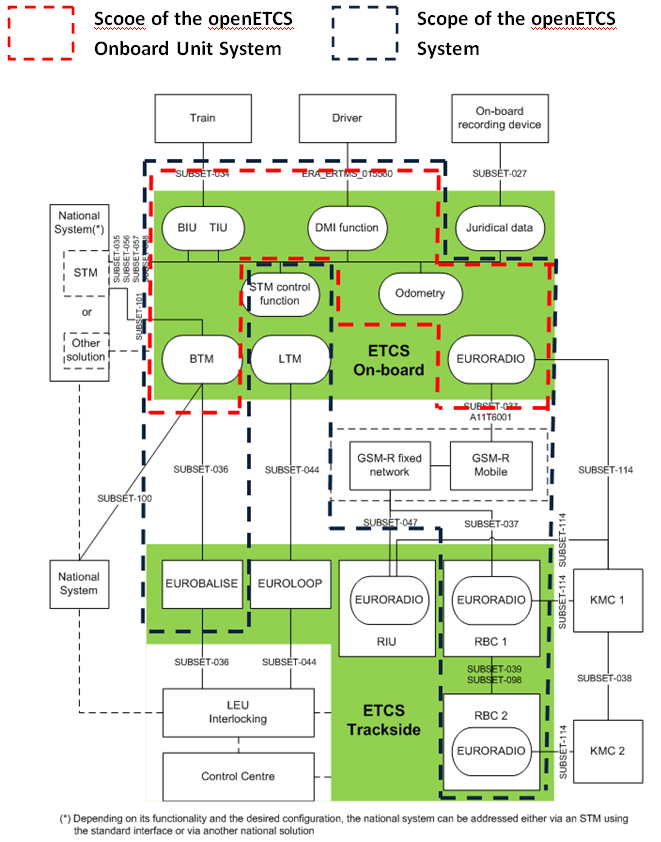
\includegraphics[width=.9\linewidth]{./images/ArchitectureSRS.PNG}
\caption{\label{fig:openETCSSystemOfInterest}OpenETCS system of interest (dotted black line) to cover demonstration objective of ITEA2 project and according to ERA TSI Chapter 2}
\end{figure}

\section{OpenETCS design process (WP3) and design artifacts}
\label{InterestOfReferenceEngineeringArtefacts}
After recalling the development process and precising openETCS project scope we must now look at the design process to see which artifacts are produced to meet openETCS requirements. This process is under WP3 responsibility.

\label{DesignProcessStrategy}

At system level (ETCS), we have to produce two main specifications: Elaborated System Requirements Specification and System Architecture Design Specification.

First idea would be to formalize SRS subset 026 on the scope defined previously and then continue system decomposition from this formalization but from experience of openETCS partners, this approach \textit{is not sufficient in order to fully understand the main issues that stem from the approach by which the SRS was conceived}.

So, instead of building yet another copy-paste direct formalisation of the ETCS SRS, WP3 suggested another approach using a SRS functional analysis centred on Onboard unit (instead of EVC) and focused on the reference track (ETCS L2 Utrecht- Amsterdam).

This approach leads to the following architecture and design artifacts described in \cite{ArchitectureDesignSpecification} :
\begin{itemize} 
\item User story models that refine textual user stories about use of OBU in operational context: done with SysML language and Papyrus tool. It provides another entry for project stakeholder requirements and prepares validation.
\item System Architecture model, defined with SysML language and Scade system Designer tool, with currently two decomposition levels: 
		\begin{itemize} \item System breakdown structure, centred on ETCS OBU and defining required interactions to other ETCS subsystems (external interfaces)
		\item Functional breakdown from OBU, centred on ETCS Kernel and defining functional interactions between those internal functions (internal interfaces)
		\end{itemize} 

\item OpenETCS application software executable model, a model defined with SCADE tool by integration of several functional block models that realize functional block interfaces identified and characterized in Architecture model
\item Environment model, designed with SCADE tool and SCADE display for simulation HMI, that supports validation of OpenETCS application software executable model
\item OBU SW Architecture and Design Document (ADD) providing a functional description of software architecture and design
\item A RFC (Request For Comment) process that provides a cross-reference to the SRS, listing
all requirements and design conflicts that have been identified during work. 

\end{itemize}

Figure \ref{fig:OpenETCSArchitectureAndDesignModel} illustrates the architecture breakdown performed in openETCS architecture model starting from ETCS system down to ETCS kernel software component.


\begin{figure}[htbp]
\centering
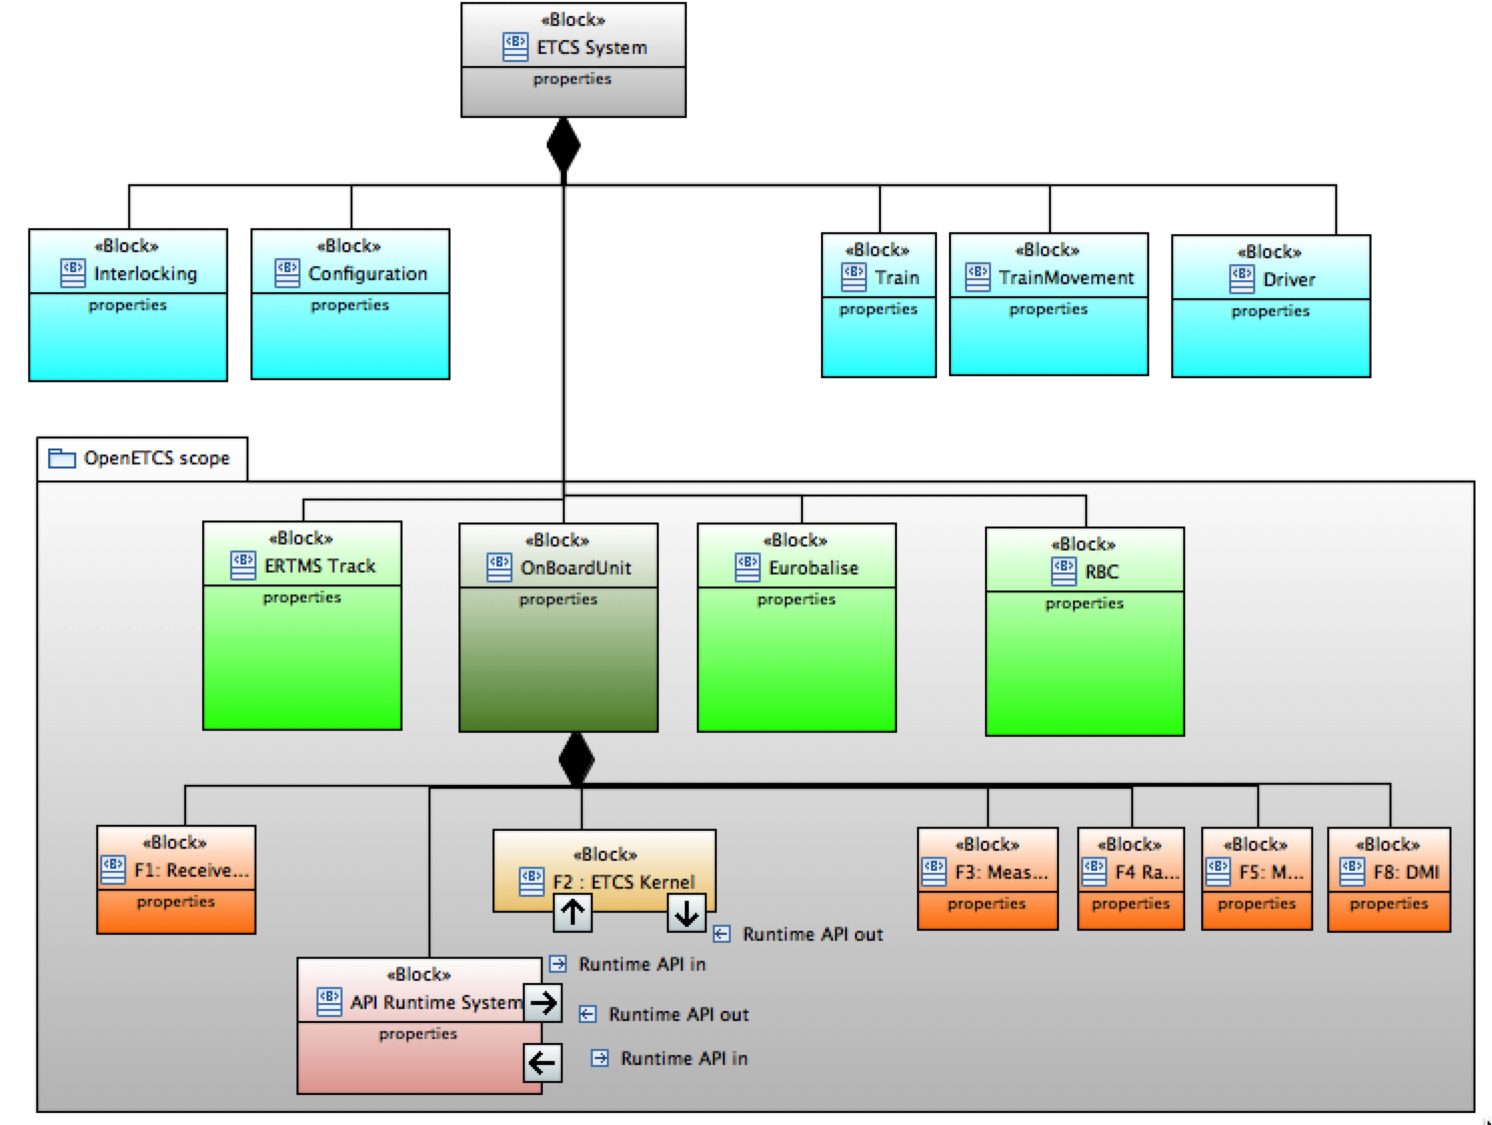
\includegraphics[width=.9\linewidth]
{./images/OpenETCSArchitectureAndDesignModel.png}
\caption{\label{fig:OpenETCSArchitectureAndDesignModel}OpenETCS architecture with SysML: from system to software components}
\end{figure}

Figure \ref{fig:WP3DesignProcess} summarises design process defined by WP3 and shows relations between different design documents and with reference input artifacts: SRS subset26, Utrech-Amsterdam reference track scenarios and openETCS API for platform interoperability. Black arrows mean "input for" while red arrows are traceability relations to reference artifacts.

\begin{figure}[htbp]
\centering
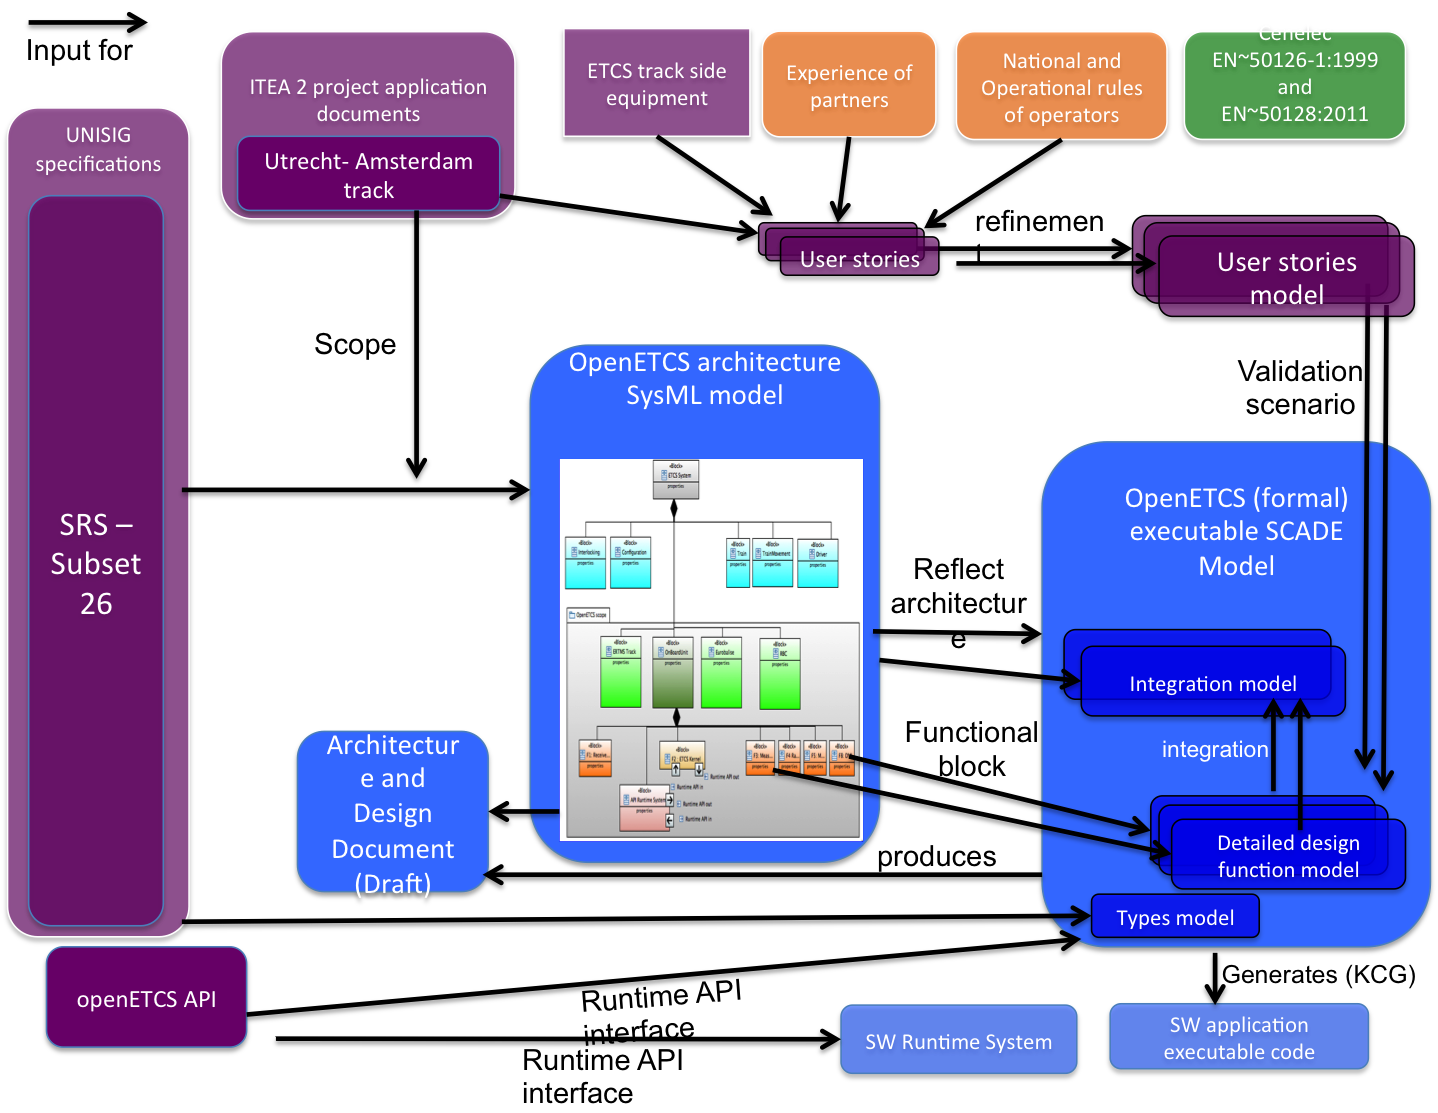
\includegraphics[width=1.0\linewidth]
{./images/WP3DesignProcess.png}
\caption{\label{fig:WP3DesignProcess}Relations between main WP3 Design Documents and reference input artifacts (SRS, Utrecht-Amsterdam reference track and OpenETCS API)}
\end{figure}

\section{OpenETCS VV and safety process (WP4)}


\cite{D4.2.3} recalls that the openETCS software development has to interact with a respective generic safety management process and take the overall safety requirements for a train control system into account. 

During validation of product, OpenETCS project has to provide a safety case. 
The openETCS safety case shall present a transparent and easy to follow argumentation chain
connecting the system definition with all basic safety assumptions and all evidence. To do this it
has to show the relations between design and V\& V artifact created during the iterative openETCS
development process. Thereby, it has to be shown to which degree and under which assumptions
the resulting documentation covers process, quality and safety requirements based on EN 50126,
EN 50128 and EN 50129.

Figure \ref{fig:SafetyProcess} shows the interactions between design, verification and validation and the general quality and safety management.

\begin{figure}[htbp]
\centering
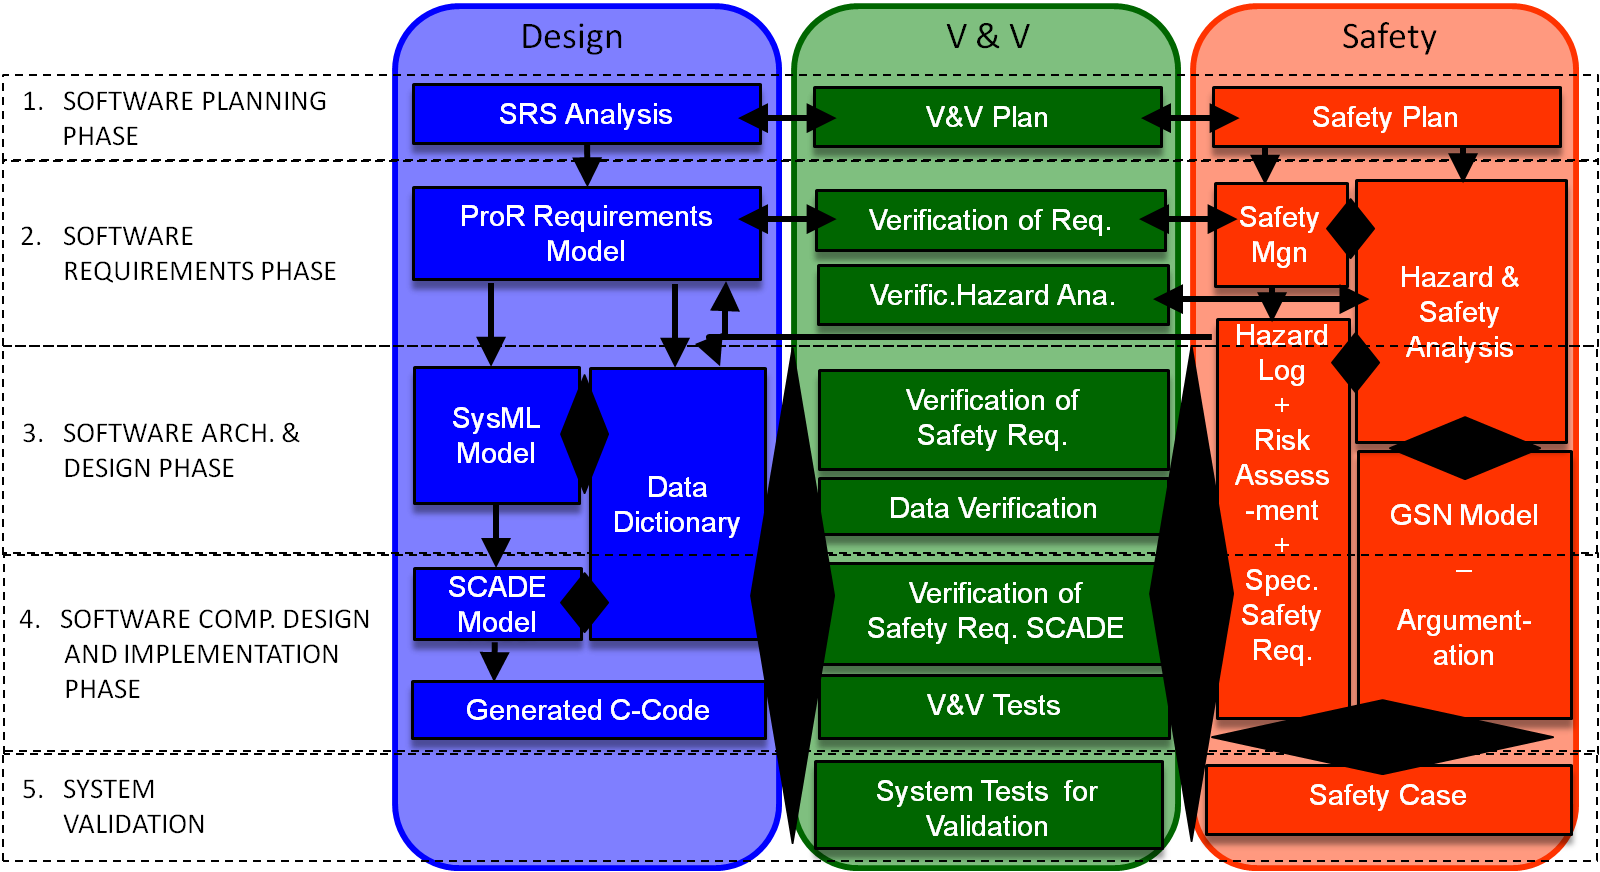
\includegraphics[width=1\linewidth]{./images/openETCS-Software-Safety-Development.png}
\caption{OpenETCS development relations between design, verification and validation and safety activities}
\label{fig:SafetyProcess}
\end{figure}




\chapter{OpenETCS traceability priorities and detailed expectations}

\section{Traceability main priority from WP3}
From WP3 point of view, most important traceability chain concerns links between ETCS OBU formal model and Subset026 SRS requirements and all other requirements created during system analysis, either by decomposition, refinement or derivation. 
ETCS OBU model is detailed down to software detailed design level, and as it is a formal model, it becomes possible to generate code from that model. So, if it is possible to demonstrate that this model satisfies some Subset026 SRS requirements, then it will be possible to establish that software code generated from that model also satisfies those requirements.

Figure \ref{fig:openETCSTraceabilityMainPriority} highlights traceability chains with highest priority (arrows with largest size).

\begin{figure}[htb]
\centering
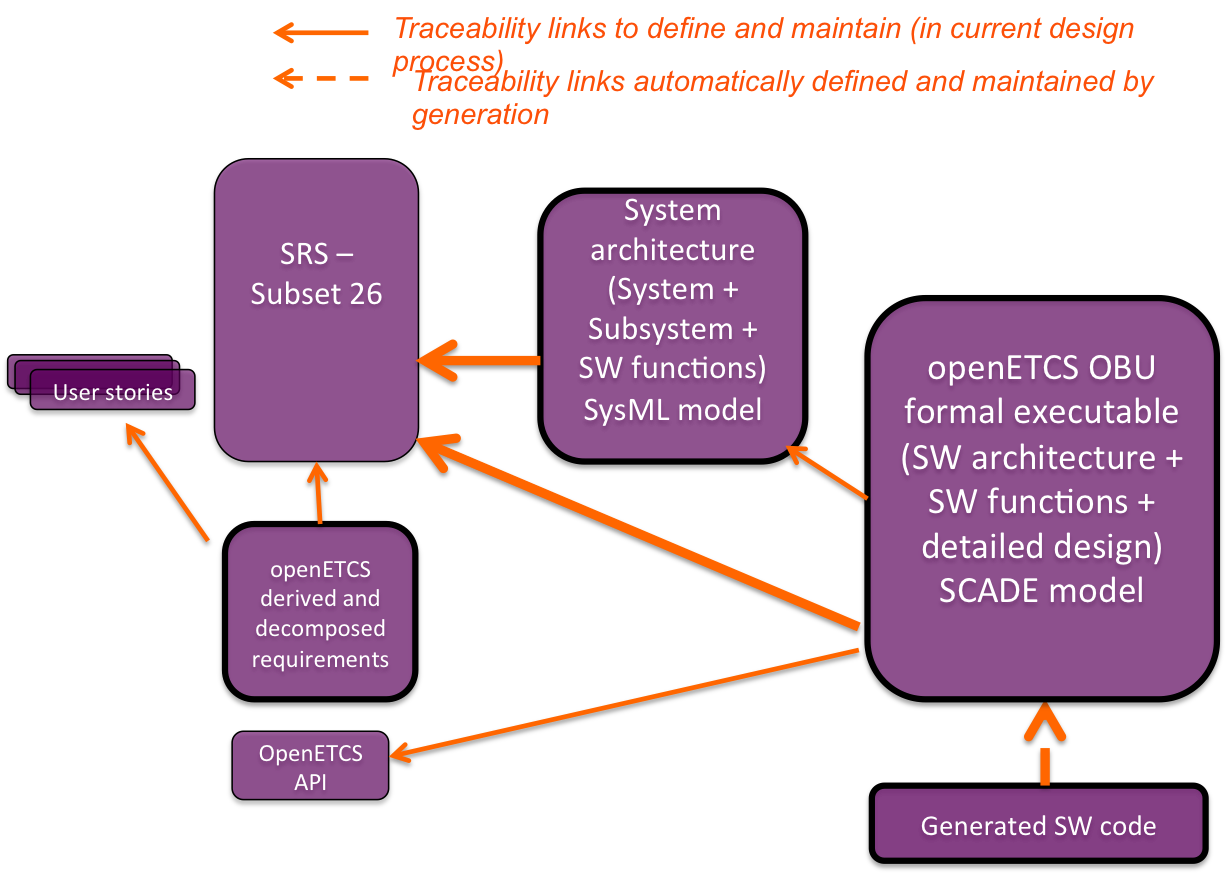
\includegraphics[width=.9\linewidth]
{./images/openETCSTraceabilityMainPriority.png}
\caption{\label{fig:openETCSTraceabilityMainPriority}OpenETCS traceability chains with highest priority}
\end{figure}

Next paragraphs explain traceability during the 5 phases of the software development process with specific focus on links between openETCS OBU model and SRS Subset 26.



\section{OpenETCS traceability main scenarios}
Traceability main scenarios are grouped by phase according to the openETCS software development process introduced in previous chapter. We recall it below to ease reading of next paragraphs.

\begin{figure} [htbp]
\centering
\includegraphics[width=.9\linewidth]
{./images/OpenETCSDevelopmentProcess.png}
\caption{\label{fig:OpenETCSDevelopmentProcess}OpenETCS software development process}
\end{figure} 

\subsection{P1 Software specification Phase}

P1 covers requirement development activities for software development.
Figure \ref{fig:P1RequirementDerivation} shows requirement derivation process from reference stakeholder requirements that make the OpenETCS baseline down to SW requirements.


\begin{figure}[htbp]
\centering
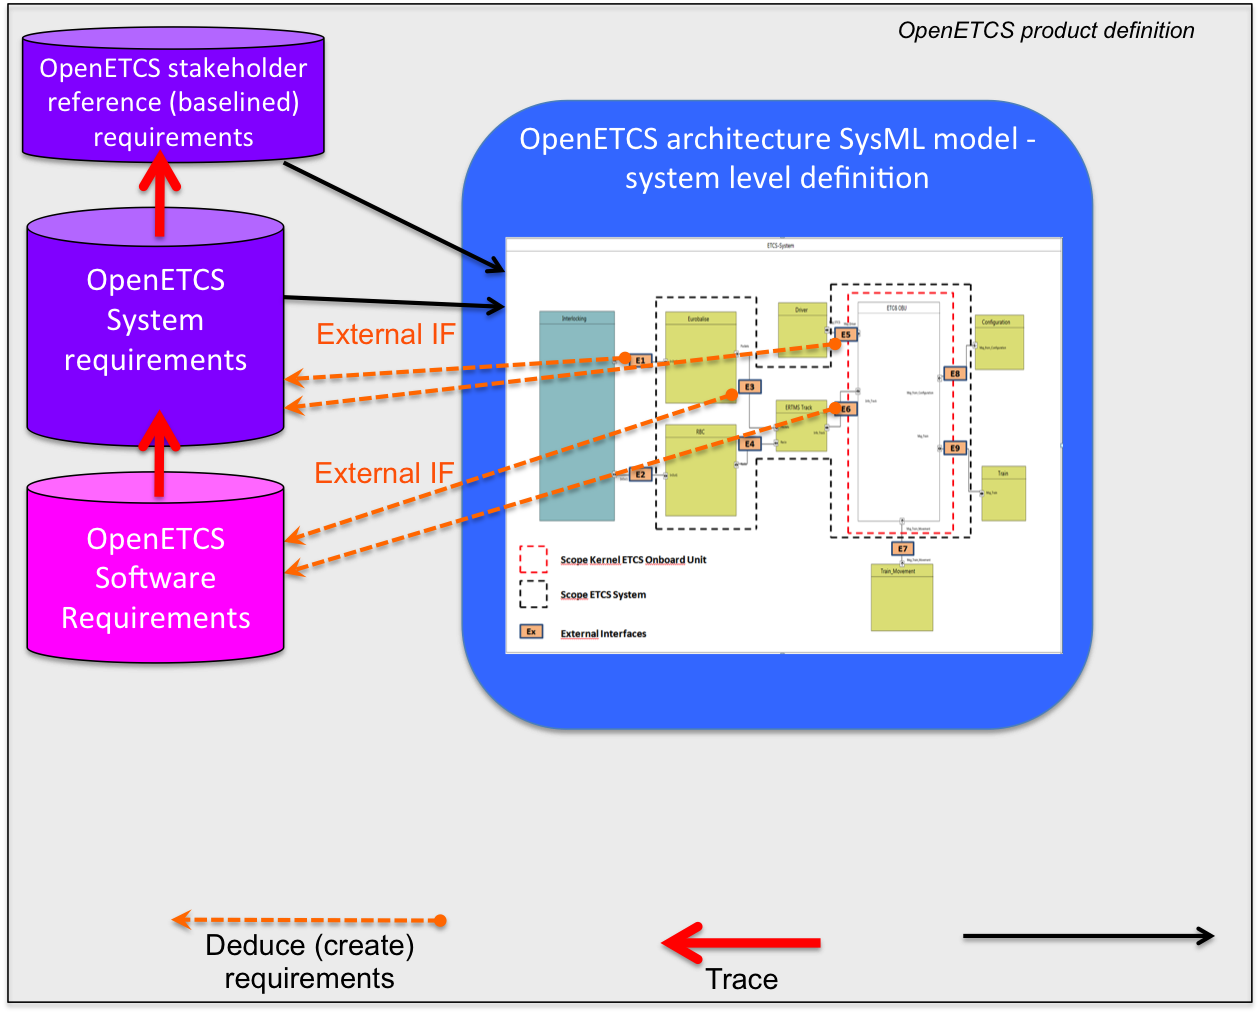
\includegraphics[width=.9\linewidth]
{./images/P1RequirementDerivation.png}
\caption{\label{fig:P1RequirementDerivation}Requirement derivation process down to software requirements with traceability}
\end{figure}

Software Overall Test Specification will be derived with respect to software requirements, but a method is not defined at this point.

The main part of input system derivation process from SUBSET 26 to software requirements is done through SysML architecture model as illustrated in figure \ref{fig:P1RequirementDerivationWithSysMLModel}.
 
We do not detail this activity and associated traceability because it is not current priority. However, this derivation process remain important in order to ensure good relevance of software requirements with regards to SUBSET 26 and other system specifications.

\begin{figure}[htbp]
\centering
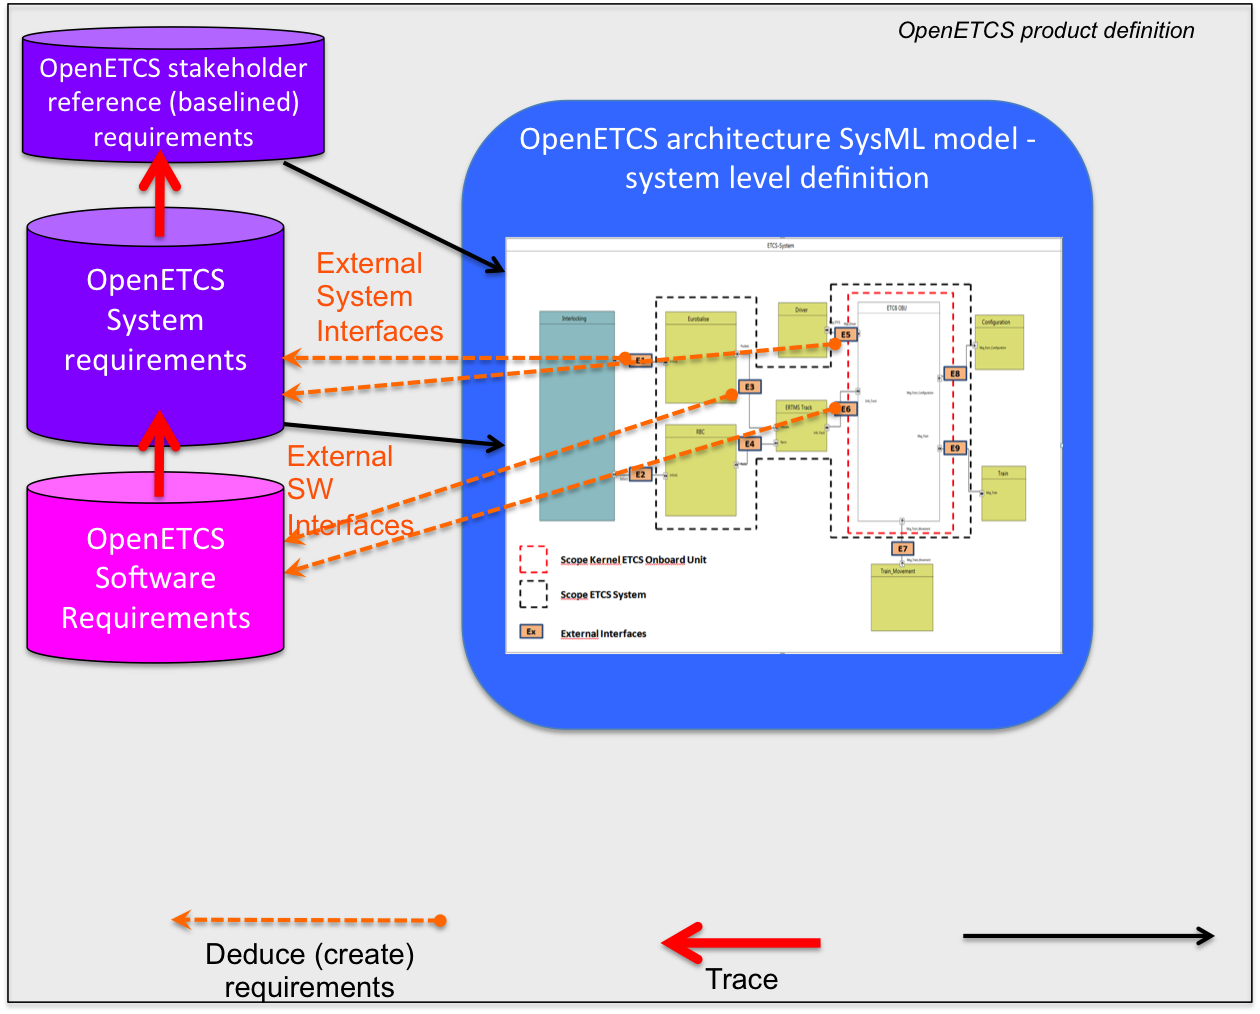
\includegraphics[width=.9\linewidth]
{./images/P1RequirementDerivationWithSysMLModel.png}
\caption{\label{fig:P1RequirementDerivationWithSysMLModel}Requirement derivation process through SysML architecture model}
\end{figure}


\subsection{P2 - Software Architecture Modeling Phase}
The phase P2 covers activities from the EN~50128 development life cycle Software Arch. \& Design Phase (7.3).

The SysML model initiated in P1 is completed to represent the Software Architecture specification. It is reflected into a SCADE model that will be used for integration (as the overall SCADE model is composed of several components described by SCADE models and the defined interfaces, the integration is performed and documented in the SCADE model).

Figure \ref{fig:P2SoftwareArchitectureWithSysMLModel} summarizes those activities and associated artifacts.

\begin{figure}[htbp]
\centering
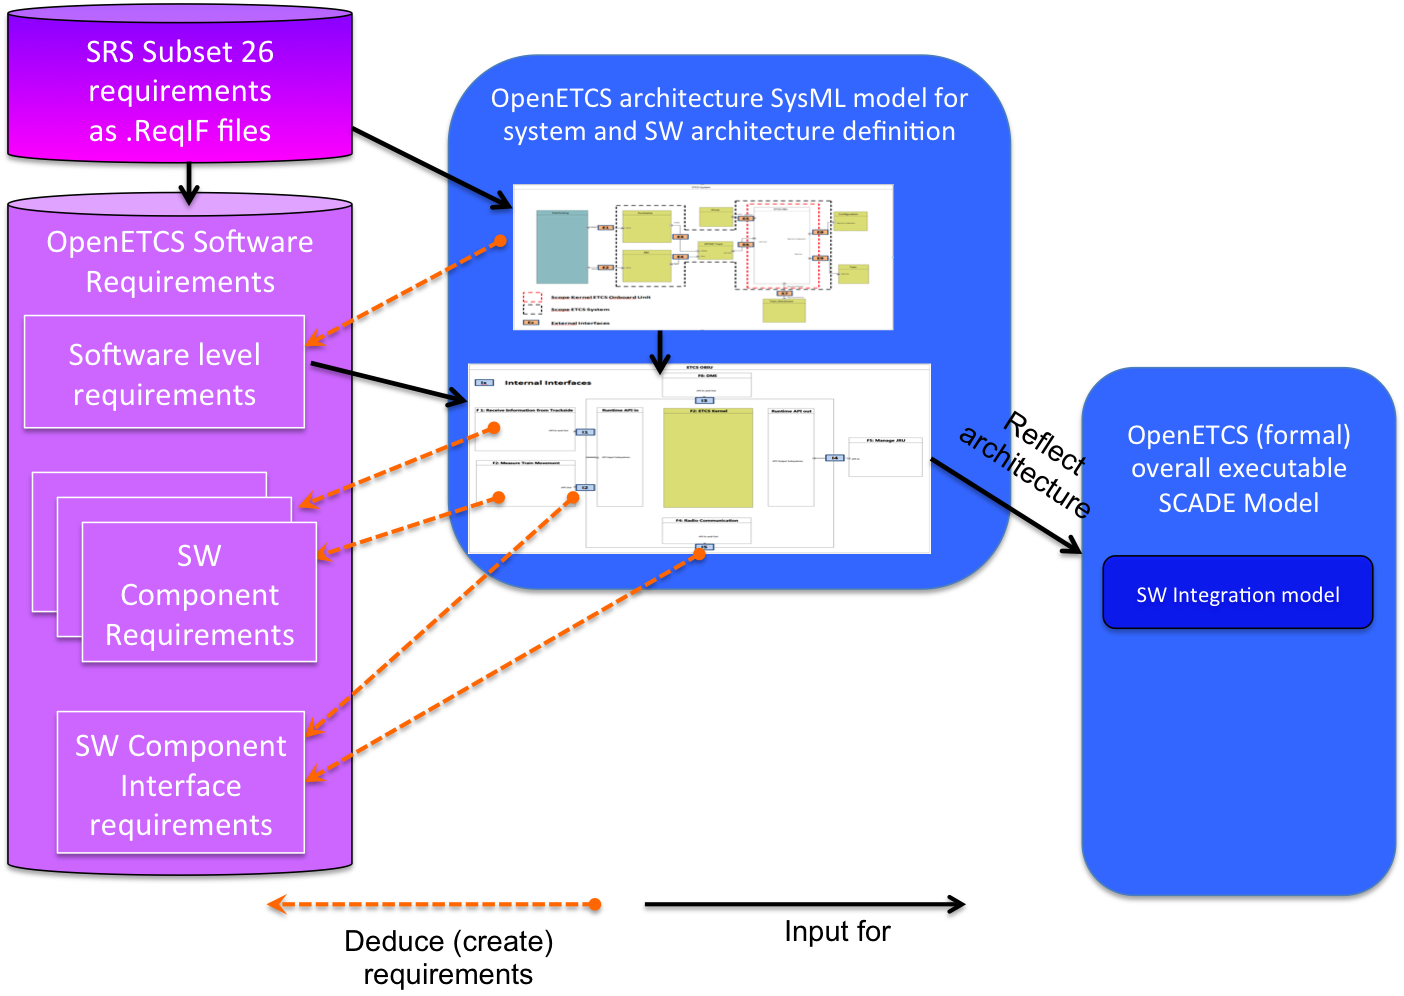
\includegraphics[width=.9\linewidth]
{./images/P2SoftwareArchitectureWithSysMLModel.png}
\caption{\label{fig:P2SoftwareArchitectureWithSysMLModel}Software architecture definition through SysML model}
\end{figure}



\subsection{P3 - Software Behavior Modeling and Integration Phase}

The phase P3 \textit{Software Behavior Modeling and Integration Phase} cover activities from the EN~50128 development life cycle Software Arch. \& Design Phase (7.3), Software Component Design Phase (7.4) and Software Component Implementation Phase (7.5). 
The SCADE model is refined and enhanced to completely represent Design and Interface Specifications as well as all Component Design Specifications. Source Code in C is generated automatically via the certified SCADE Code Generator and combined with required wrapper software. For these wrapper parts specific development methods have to be defined as these parts are specified.

\textit{Figure toDo.\textbf{•}}


\subsection{P5 - Formal Validation Phase}

The phase P5 has to cover activities of the Software Component Testing Phase (7.5), Integration Phase (7.6) and mainly Software Validation Phase (7.7) by using simulation, testing and model checking methods. To do so the SCADE environment as well as additional tools are use depending on the specific model property to be tested or proven. 

The Inputs for these activities are the SysML and SCADE models and the C Code.

\textbf{To complete}

\chapter{OpenETCS tool chain requirements about traceability}
\label{sec-4} 
Requirement traceability cannot be fully supported by tool chain if there is no ability to manage requirements (create, edit, visualize, classify...) as expressed in previous chapter through traceability process and main scenario.
Next paragraphs define tool chain capabilities required to support requirement management and requirement traceability in the context of OpenETCS expectations presented previously.

\section{Tool chain capabilities to support requirement management}

Requirement management is an activity that consists in supporting different tasks concerning requirements during the project, whatever the engineering level. In OpenETCS project we need at least the following commands available in the tool chain (and potentially restricted according to access rights if defined):
\begin{itemize}

\item Visualization of one or several requirements, their links if any and their attributes. 
\begin{itemize} \item \textbf{OpenETCS example}: visualize one Subset026 SRS or API requirement, its statement and its hierarchy (father requirement if any and children requirements if any).
	\item \textbf{OpenETCS example}: visualize one openETCS software requirement, its statement and upstream traces up to Subset 026.\end{itemize}

\item Query (filter, ordering) on a set of requirements with filter based on requirement attribute values or on links between requirements
\begin{itemize} \item \textbf{OpenETCS example}: list only subset026 SRS chapter 7 requirements that are not yet traced (no traceability link)	\item \textbf{OpenETCS example}: list OpenETCS SW requirements that are not yet traced (no traceability link).
\end{itemize}

\item Creation and storage of requirement and of different attributes based on a given requirement template/type, in a given requirement hierarchy and with unique identifier allocation based on a flexible (customizable) strategy
\begin{itemize} \item \textbf{OpenETCS example}: creation of a new openETCS requirement decomposed from a susbet026 SRS requirement, from risks and hazards analysis (safety requirement) or from software design. Newly created requirement shall have unique identifier automatically allocated to be consistent with its hierarchy (father requirement id) and with an attribute "maturity" set to "to be confirmed" and creation date set to the current date.
\end{itemize}

\item classification of one or several requirements into engineering levels (scopes) that can be defined by end users.
\begin{itemize} \item \textbf{OpenETCS example}: allocation of a newly created requirement to the OpenETCS system level, Onboard Unit SW level, OB SW component level or OBU SW component interface level .\end{itemize}

\item Edition of one or several requirements and their attributes
\begin{itemize} \item \textbf{OpenETCS example}: confirmation of a newly created requirement with attribute "maturity" set to "confirmed".\end{itemize}

\item Addition of a version on one requirement or on a set of requirements
\begin{itemize} \item \textbf{OpenETCS example}: selection of a set of reviewed openETCS requirements of a given scope (level) and addition of a version for all those requirements.\end{itemize}

\item Ability to compare two versions of a set of requirements and list all requirements that have been added or modified.
\begin{itemize} \item \textbf{OpenETCS example}: comparison of two versions of Subset026 SRS requirements (system input activities) or two versions of OBU SW requirements and visualization of all requirement links to check.\end{itemize}

\item Import of requirements coming from external sources (ReqIF, Word, Excel...)
\begin{itemize} \item \textbf{openETCS example}: import of Subset026 Word document (System specification activities) or ReqIF format (OBU SW requirements). Import of openETCS API definition.\end{itemize}

\item Export of a set of requirements to another format: at least ReqIF standard interchange format but also office format (.csv, excel or word...) \begin{itemize} \item \textbf{OpenETCS example}: export of all openETCS created requirements and links into .csv file \end{itemize}

\end{itemize}

In addition, requirement management tooling shall enable share and access of requirements within a team, through a shared repository (shared directory on a network drive or CVS repository like SVN, Git, ClearCase or any other one): either directly (all team members access same shared repository) or with local work and synchronizations between team members through a shared repository.

\section{Tool chain capabilities to support requirement traceability}
\label{sec-3-2}  
Requirement traceability activity consists in ensuring that all product engineering artifacts (including verification means) can be traced to an originating stakeholder requirement either directly (direct link) or through other requirements derived from stakeholder requirements. It means creating links but also manage their status (created, confirmed...) and potentially their deletion.

In order to support this activity in openETCS project we need at least the following commands available in the tool chain:

\begin{itemize}

\item Creation of a link between a requirement and an engineering artifact, based on a given link template/type (refine, derive, implement, verify...). 
\begin{itemize} \item \textbf{OpenETCS example}: create a "Satisfy" link between one openETCS SW functional requirement and one OnBoard Unit function, with  "status" link attribute set to "defined" and "rationale" attribute set with appropriate justification.\end{itemize}

\item edition of link status. 
\begin{itemize} \item \textbf{OpenETCS example}: after review, confirm some traceability links  by setting "status" attribute to "validated" value.
	\item \textbf{other OpenETCS example}: after change in some openETCS SW requirements, for all traceability links of modified requirements, set status to "to check" value.\end{itemize}

\item deletion of requirement traceability link. 
\begin{itemize} \item \textbf{OpenETCS example}: after review, decide that some traceability links are not accurate and delete them.\end{itemize}

\item export of requirement traceability
\begin{itemize} \item \textbf{OpenETCS example}: after progress meeting, export current requirement traceability to .csv file so that it can be analyzed by project manager and/or quality team\end{itemize}

\end{itemize}

\chapter{Tool chain current physical architecture solution to support traceability}
\label{sec-5}
\section{Overview of current traceability architecture solution}
This current solution consists in handling requirement management and traceability links through different tools and technologies. The strategy of this approach consists in maximizing efficiency of the different concurrent activities through using tooling locally integrated in the different environments used in the project over its development life cycle (the 5 phases).

As a summary view (will be detailed later) we find:
- P1: ProR to support requirement derivation process with .ReqIf database, assisted of Scade System to support SysML modeling of architecture model from system environment down to software definition and its external interfaces.
- P2: Scade System again to support SysML modeling of software architecture definition with identification of software components and component interface definitions. ReqIF reference requirements are imported in Scade System with papyrus  plugin. Additional requirements are created in SysML with Scade System. Traceability links are created in SysML with Scade System and are exported back to ReqIF database through ProR proxy. 
- P3 and P4: Scade Suite to support formal modeling of Software components and their behavior down to executable level, assisted of SCADE KCG to support generation of C source from SCADE model.
- P5: toDo

Figure \ref{fig:trace_first} illustrates current traceability architecture with associated set of tools, scripts and procedures.


\begin{figure}[htbp]
\centering
\includegraphics[width=.9\linewidth]{images/first_trace_solution.pdf}
\caption{\label{fig:trace_first}Traceability architecture first solution}
\end{figure}

\textbf{Note}: when requirement management tools complete imported requirements, they should guarantee the following rules:
\begin{enumerate}
\item The requirement's structure (hierarchy, scope) is not modified.
\item No requirement should be deleted.
\item Newly added requirements should be either a refinement, derivation or a decomposition of an existing one.
\item The identifier pattern should be respected.
\item Identifiers should remain unique.
\end{enumerate}


\section{P1 phase: ProR and Scade System}

Reference requirement input documents are converted to a set of ReqIF format files and informally analyses. The analysis specifies relationships between requirements and revises parts of the requirements to obtain a detailed and atomic abstraction level matching the different requirement engineering levels required by Cenelec standards. 

A script is in charge of converting input reference documents to initial set of stakeholder requirements in .ReqIF format files. See \label{importScript} for detailed description of this script, challenges to solve and solutions.

ProR is the tool in charge of supporting the requirement classification and derivation activities from this initial set of requirements and down to software requirements ReqIF files. 
\begin{itemize} 
\item It supports requirements classification into different engineering levels: stakeholder, system and software.
\item It supports creation of additional requirements coming from hazard and risks analysis (safety requirements) or coming for decomposition (improvement of requirement quality)
\item It supports creation of requirements derivation links between engineering levels.
\end{itemize}


With that approach, there is one master reference requirements data base. This data
base is itself directly imported from the subset-026 word document. The data
base provides the list of requirements as well as an unique identifiers for each
requirement. These identifiers are fixed and cannot be modified by any other
tools. 


\subsection{Script description}
\label{importScript}
The script \todo{The script needs a name} generates a hierarchical tree of all traceworthy
artifacts in each chapter of subset-026. Each artifact shall be uniquely
addressable via a tracestring.


\subsection{Unique ID definition}
\label{sec-5-1-2}
Take the following example:
\begin{figure}[htb]
\centering
\includegraphics[width=.9\linewidth]{images/tracestring-ex.png}
\caption{\label{fig:reqID_ex}Traceability architecture between artifacts}
\end{figure}


\paragraph{Guideline}
The scope of a single requirement ID is a paragraph of text (there are six such
paragraphs in the above example).  requirement IDs are hierarchical. The
hierarchy is a direct mapping of the hierarchy in the original subset-026
text. Levels are separated by a dot. There is a requirement at each level
(i.e. you may truncate the requirement ID to any level and it stays valid).

\paragraph{How to}

Suppose we want to trace the fifth paragraph in the above example i.e
\begin{verbatim}
• End of mission is performed
\end{verbatim}
\begin{enumerate}
\item Let \textsl{traceString} be the variable to store the result.
\item Find the current running number of the base list. That is the list which
includes the chapter number. In this example this number equals
\verb+3.5.3.7.+ Set \textsl{traceString} to this number.
\item Count the number of paragraphs in this list item starting with 1 and append
this number in square brackets to the \textsl{traceString} if it is greater than 1.

Note: For the first iteration in the example there is only one such paragraph
(\texttt{If the establishment...}). Hence, we do not append anything. In the
second iteration there are two such paragraphs (\texttt{The on-board shall...} and
\texttt{If this request is not ...}). Hence, the second one will receive an
\texttt{[2]} appendix.

\item Until you arrived at your target paragraph: Append any running number of
sub-lists and remove leading or trailing characters (such as braces). If the
current sub-list is bulleted then the level string always becomes
\verb+[*][n]+ (with n being the running number of that bullet starting at
1). Prefix this new level with a dot (\verb+.+) and append it to the
\textsl{traceString}.

Note: \verb+a)+ is the identifier of one such sub-list item. The trailing brace
will be removed. The bullet points form another (less significant) sub-list.
\item Do step 3.
\item Do step 4 or break.
\item \textsl{traceString} is now the fully qualified requirementID.
\end{enumerate}

This will result in the following requirement ID: \quad \verb+3.5.3.7.a[2].[*][2]+



\subsection{System Model}
\label{sec-8}

The link with the requirement may be included via requirements diagram with a
direct link of requirement in ProR
The explanation to performs the link may be found here \href{https://github.com/openETCS/toolchain/wiki/User-Documentation#tracing-requirements-and-sysml-models}{ProR-Papyrus proxy}.
The links may be viewed through Papyrus an ProR and the requirement may be
directly apply from ProR to a Papyrus elements.


\section{P2 phase: ProR, Scade System and Scade suite}

\textit{To complete}

\subsection{Transformation of SysML architecture model to SCADE architecture Model}
\label{sec-9}

It should define the interfaces between the architecture artifacts.  It is used and
set up to facilitate team working together on a big architecture. Its definition
comes from the requirements but can also be refined by the modelling team without
changing the existing implemented requirements.


\section{P3 and P4 phases: ProR, Scade suite and Scade KCG}
ToDo

\section{P5 phase: XXX}
ToDo

\chapter{Limits of current traceability architecture and axes of investigation for improvement}
\label{sec-6}

\section{Current identified limits}
ToDo

\section{Investigation axes for improvements}

\subsection{Alternative Requirement management and traceability tools}
Concerning requirement management and traceability there exist a lot of solutions. If we focus on open source solutions and especially those able to integrate into Eclipse platform, we find:
\begin{itemize}
\item Eclipse Requirement Modeling Framework (RMF). As mentioned on Eclipse web site, RMF is a framework to manage textual requirements through ReqIF standard requirement exchange format. There is a powerful GUI called "ProR" to configure, visualize and edit ReqIF requirements in RMF.
RMF/ProR is the natural choice for OpenETCS to support requirement management.

Alternatively to deal with the closed source path the requirement management may
be done by Reqtify Gateway of SCADE (also called "RM Gateway"). 

ProR can also be used to support traceability between requirements (native functionality) and between requirements and Papyrus models through a "proxy" connector.

\item PolarSys ReqCycle. It is a solution that focuses on requirement traceability. It can allow managing requirements (creation, edition, queries) with classification (scopes) and custom requirement data models but with very limited requirement editor. Strength is its ability to capture and aggregate traceability links coming from different sources (EMF models, C code, Java code, SysML models...) and to define own traceability links based on custom link types with potential attributes.

\end{itemize}

If we extend search to proprietary solutions, we find IBM DOORS and IBM DOORS Next requirement management products and Dassault Systems ReqTify product as leading solutions to support respectively requirement management and requirement traceability.

This second solution consists in using only one centralized Requirement database (as in solution 1) managed by one eclipse-based requirement management solution (ProR) and only one eclipse-based technology to support requirement traceability for all models (Papyrus and SCADE): PolarSys ReqCycle.

\begin{figure}[htb]
\centering
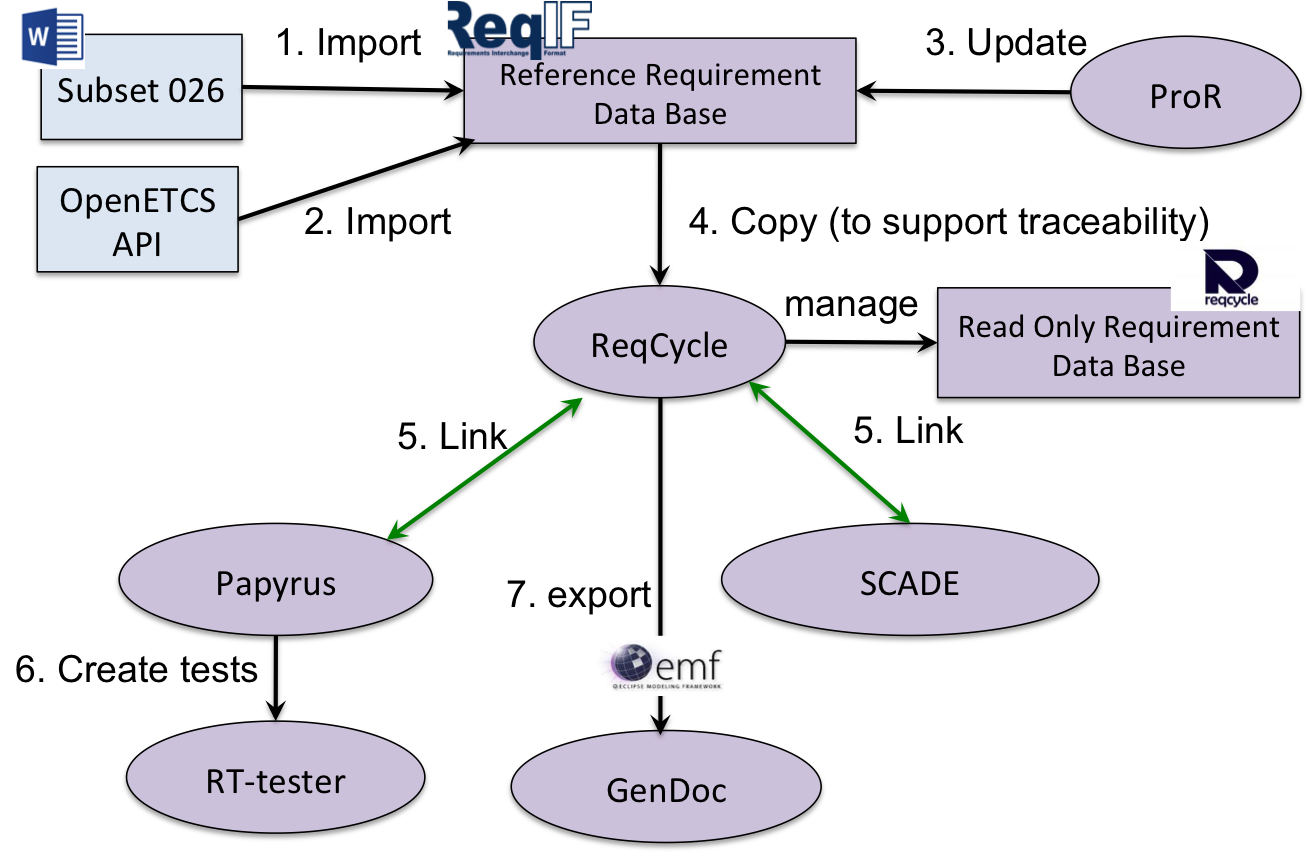
\includegraphics[width=.9\linewidth]{images/second_trace_solution-ProR-ReqCycle.png}
\caption{\label{fig:trace_second}Traceability architecture second solution}
\end{figure}

With that approach, there is still one master reference requirements data base entirely managed by ProR. Requirement database is initialized by import from the subset-026 word document, as in solution 1 (see \ref{sec-5-1}) and by import from OpenETCS API.
All new OpenETCS requirements are added in this requirement database through ProR tool.

Traceability is managed by ReqCycle tool. In order to ease visual selection of requirements in ReqCycle, there is a copy (could be a link) of reference requirements hierarchy into a ReqCycle database. Then ReqCycle manages links with Papyrus and links with SCADE. 
Finally, traceability can be exported by ReqCycle and processed by Gendoc tool to deliver documentation.

Interactions through the tool chain are detailed in figure \ref{fig:trace_second-interactions} below with focus put on traceability between requirements and functional model (traceability with SysML model, creation of tests and export of traceability are not shown here). 



\subsection{Third alternative traceability solution: ReqCycle}

This third solution consists in using only one centralized Requirement database (as in previous solutions) managed by one eclipse-based solution (ReqCycle) also used to support requirement traceability for all models (Papyrus and SCADE).

\begin{figure}[htb]
\centering
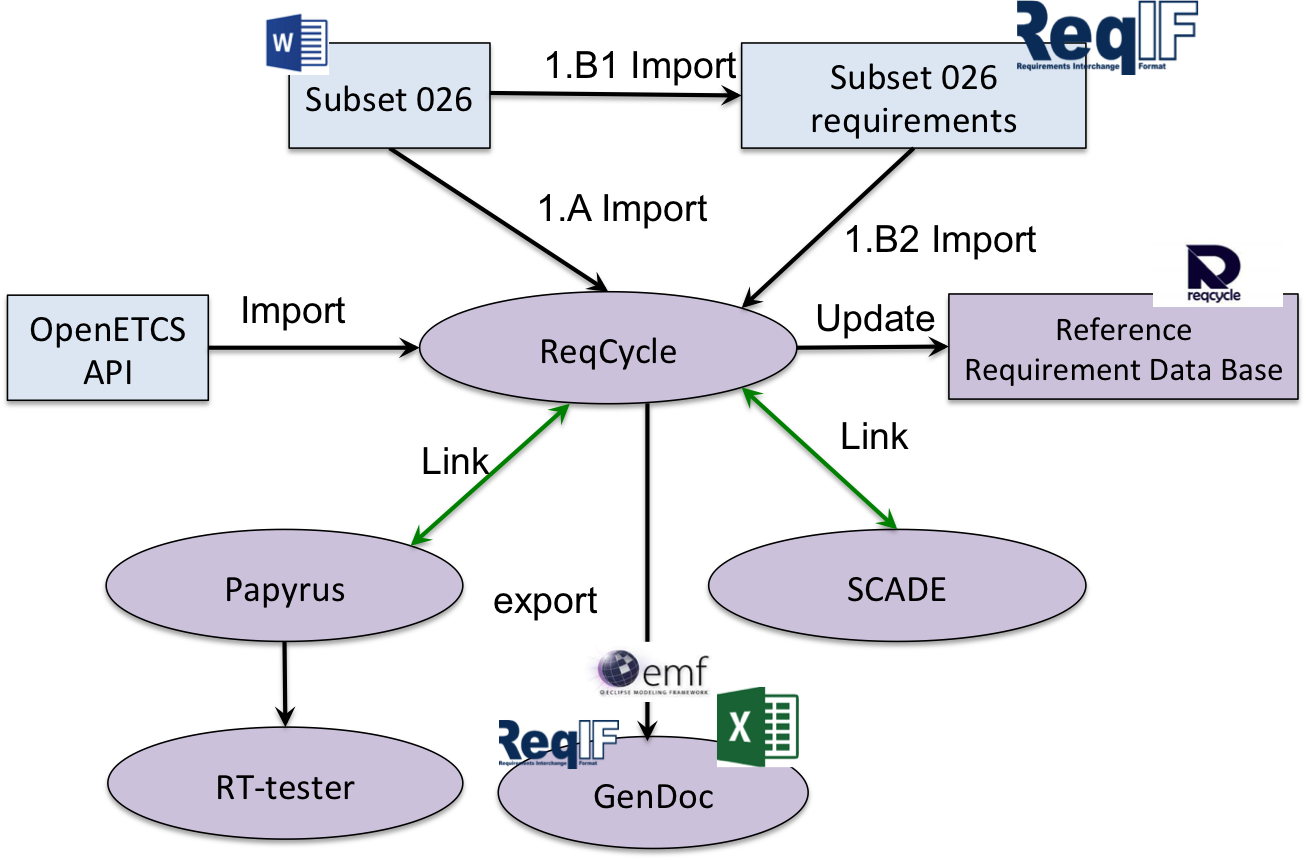
\includegraphics[width=.9\linewidth]{images/Third-Solution-ReqCycle.png}
\caption{\label{fig:trace_third}Traceability architecture third solution with ReqCycle only}
\end{figure}

With that approach, there is still one master reference requirements data base entirely managed by ReqCycle. Requirement database is initialized by import from the subset-026 word document through two possible means (see next section) and by import from OpenETCS API.
All new OpenETCS requirements are added in this requirement database through ReqCycle tool.

Traceability is managed by ReqCycle tool. In order to ease visual selection of requirements in ReqCycle, there is a copy (could be a link) of reference requirements hierarchy into a ReqCycle database. Then ReqCycle manages links with Papyrus and links with SCADE. 
Finally, traceability can be exported by ReqCycle and processed by Gendoc tool to deliver documentation.




%% Bibliography
% \nocite{*}
\bibliographystyle{unsrt}
\bibliography{oetc_WP7_Traceability}



%Examples are below


%\lipsum[11]

%\nocite{*}

%\bibliographystyle{unsrt}
%\bibliography{Lbrr}



% \begin{thebibliography}{9}

% \bibitem{lamport94}
%   Leslie Lamport,
%   \emph{\LaTeX: A Document Preparation System}.
%   Addison Wesley, Massachusetts,
%   2nd Edition,
%   1994.

% \end{thebibliography}

%===================================================
%Do NOT change anything below this line
\end{document}

%%  LocalWords:  traceability OpenETCS
